\section{R Primer} 



\subsection{Installation}

 	%==============================================================================================%
	\begin{frame}
		\frametitle{R Installation}
	\begin{itemize}
		\item R is available as binaries \& source code for Windows, Mac and Linux
		\item \url{https://ftp.heanet.ie/mirrors/cran.r-project.org/}
	\end{itemize}
	However, R is also packaged within Rstudio
	\begin{itemize}
		\item open-source, IDE for R
		\item very user-friendly
		\item https://www.rstudio.com/products/rstudio/download/
	\end{itemize}
	\end{frame}

 	%==============================================================================================%
 	\begin{frame}[fragile]
	\frametitle{Let's spend some time checking our installation}
 		% % SLIDE 1 - COVER SLIDE
		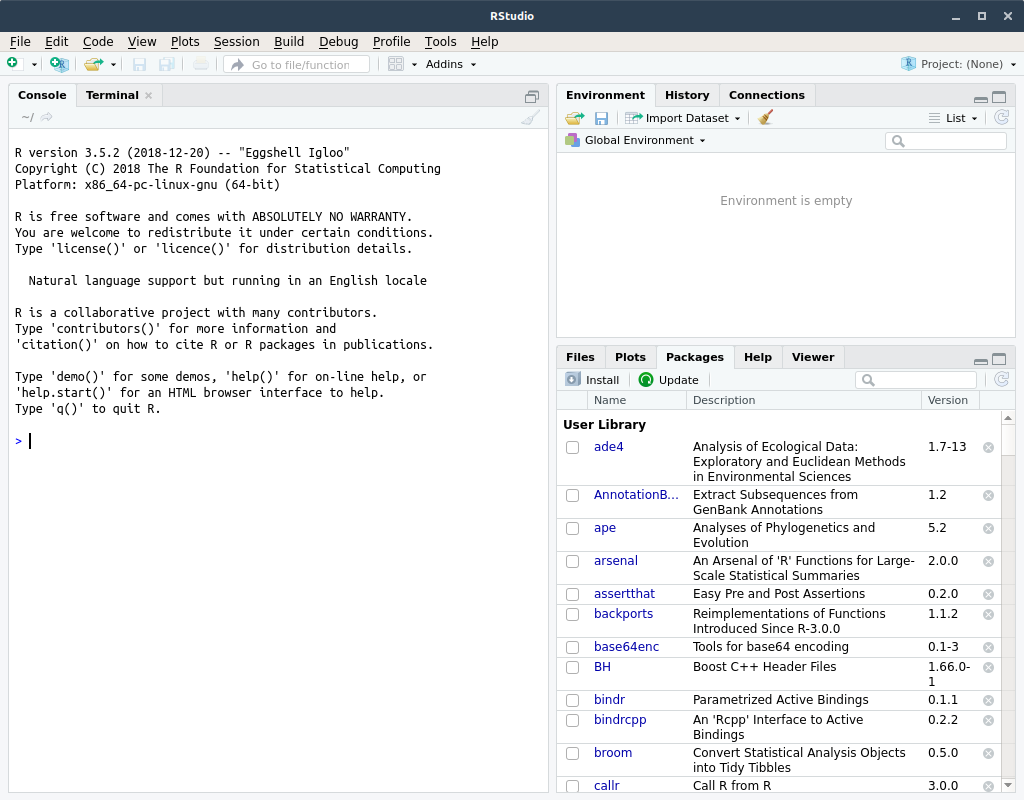
\includegraphics[scale=0.2]{./figures/rstudio}
 	\end{frame}
 	

 	
